\documentclass[12pt, twoside]{article}
\documentclass[12pt, twoside]{article}
\usepackage[letterpaper, margin=1in, headsep=0.2in]{geometry}
\setlength{\headheight}{0.6in}
%\usepackage[english]{babel}
\usepackage[utf8]{inputenc}
\usepackage{microtype}
\usepackage{amsmath}
\usepackage{amssymb}
%\usepackage{amsfonts}
\usepackage{siunitx} %units in math. eg 20\milli\meter
\usepackage{yhmath} % for arcs, overparenth command
\usepackage{tikz} %graphics
\usetikzlibrary{quotes, angles}
\usepackage{graphicx} %consider setting \graphicspath{{images/}}
\usepackage{parskip} %no paragraph indent
\usepackage{enumitem}
\usepackage{multicol}
\usepackage{venndiagram}

\usepackage{fancyhdr}
\pagestyle{fancy}
\fancyhf{}
\renewcommand{\headrulewidth}{0pt} % disable the underline of the header
\raggedbottom
\hfuzz=2mm %suppresses overfull box warnings

\usepackage{hyperref}
\usepackage{float}

\title{Algebra 2}
\author{Chris Huson}
\date{December 2023}

\fancyhead[LE]{\thepage}
\fancyhead[RO]{\thepage \\ Name: \hspace{4cm} \,\\}
\fancyhead[LO]{BECA / Huson / Algebra 2: Polynomials Jan 2023 Regents \\* 9 April 2024}

\begin{document}

\subsubsection*{Regents problems: Polynomials}
\begin{enumerate}[itemsep=0.5cm]
\item Which expression is equivalent to $(x + 2)^2 - 5(x + 2) + 6$? %January 2023 Regents
\begin{enumerate}
    \item $x(x - 1)$
    \item $(x - 3)(x - 2)$
    \item $(x - 4)(x + 3)$
    \item $(x - 6)(x + 1)$
\end{enumerate}

\item The expression $\displaystyle \frac{x^4 - 5x^2 + 4x + 14}{x+2}$ is equivalent to %January 2023 Regents
\begin{enumerate}
    \item $\displaystyle x^3 - 2x^2 - x + 6 + \frac{2}{x + 2}$
    \item $\displaystyle x^3 - 5x + 4 - \frac{14}{x + 2}$
    \item $\displaystyle x^3 + 2x^2 - x + 2 + \frac{18}{x + 2}$
    \item $\displaystyle x^3 + 2x^2 - 9x + 22 - \frac{30}{x + 2}$
\end{enumerate}

\item Given $x \ne -3$, which expression is equivalent to $\displaystyle \frac{2x^3 + 3x^2 - 4x + 5}{x+3}$? %August 2023 Regents
\begin{enumerate}
    \item $\displaystyle 2x^3 + 9x^2 + 23x + 74$
    \item $\displaystyle 2x^2 - 3x + 5 - \frac{10}{x+3}$
    \item $\displaystyle 2x^3 -3x^2 + 5x - 10$
    \item $\displaystyle 2x^3 + 9x + 23 + \frac{74}{x+3}$
\end{enumerate}

\item If \(f(x) = 2x^4 - x^3 - 16x + 8\), then \(f\left(\frac{1}{2}\right)\) %January 2023 Regents
\begin{enumerate}
    \item equals 0 and \(2x + 1\) is a factor of \(f(x)\)
    \item equals 0 and \(2x - 1\) is a factor of \(f(x)\)
    \item does not equal 0 and \(2x + 1\) is not a factor of \(f(x)\)
    \item does not equal 0 and \(2x - 1\) is a factor of \(f(x)\)
\end{enumerate}

\item What is the solution set of the equation \(\displaystyle \frac{x+2}{x} + \frac{x}{3} = \frac{2x^2+6}{3x}\)? %January 2023 Regents
\begin{enumerate}
    \item \(\{-3\}\)
    \item \(\{-3, 0\}\)
    \item \(\{3\}\)
    \item \(\{0, 3\}\)
\end{enumerate}

\item The graph of a quadratic function is shown below. %August 2023 Regents
\begin{center}
    \begin{tikzpicture}[scale=0.65]
        \draw[thick,->] (-6,0) -- (6.5,0) node[below] {$x$};
        \draw[thick,->] (0,-8) -- (0,6.5) node[above] {$y$};
        \draw[thin,gray!50] (-6,-8) grid (6,6);
        \draw[thick] (5pt,5)--(-5pt,5) node[left] {$5$};
        \draw[thick] (5,5pt)--(5,-5pt) node[below] {$5$};
        \draw[thick, domain=-2.5:4.5, samples=100] plot (\x, {-(\x)^2 + 2*\x + 4});
    \end{tikzpicture}
    \end{center}
Then the graph of $x + y = 4$ is drawn on the same axes, one solution
to this system is
\begin{enumerate}
    \item $(4,0)$
    \item $(1,5)$
    \item $(2,2)$
    \item $(3,1)$
\end{enumerate}

\item How many real solutions exist for the system of equations below? %January 2023 Regents
\begin{align*}
    y &= \frac{1}{4} x - 8 \\
    y &= \frac{1}{2} x^2 + 2x
\end{align*}
\begin{enumerate}
    \item 1
    \item 2
    \item 3
    \item 0
\end{enumerate}

\item Which equation represents a polynomial identity? %January 2023 Regents
\begin{enumerate}
    \item \(x^3 + y^3 = (x + y)^3\)
    \item \(x^3 + y^3 = (x + y)(x^2 - xy + y^2)\)
    \item \(x^3 + y^3 = (x + y)(x^2 - xy - y^2)\)
    \item \(x^3 + y^3 = (x - y)(x^2 + xy + y^2)\)
\end{enumerate}

\item Given $f(x) = x^4 - x^3 - 6x^2$, for what values of $x$ will $f(x)>0$? %January 2023 Regents
\begin{enumerate}
    \item $x<-2$, only
    \item $-2<x$ or $x>3$
    \item $-2<x$ or $0 \le x \le 3$
    \item $x>3$, only
\end{enumerate}

\item  Consider a cubic polynomial with the characteristics below. %January 2023 Regents
\begin{itemize}
\item exactly one real root
\item as $x \rightarrow \infty$, $f(x) \rightarrow -\infty$
\end{itemize}
Given $a>0$ and $b>0$, which equation represents a cubic
polynomial with these characteristics?
\begin{enumerate}
    \item $f(x) = (x - a)(x^2 + b)$
    \item $f(x) = (a - x)(x^2 + b)$
    \item $f(x) = (a - x^2)(x^2 + b)$
    \item $f(x) = (x - a)(b - x^2)$
\end{enumerate}

\item Which graph shows a quadratic function with two imaginary zeros? \\ %January 2023 Regents
\includegraphics*[width=8cm]{../graphics/regents-jan2023-24-polynomials.png}

\item In the quadratic formula, $b^2-4ac$ is called the discriminant. The function $f(x)$ has a discriminant value of 8, and $g(x)$ has a discriminant value of $-16$. The quadratic graphs, $h(x)$ and $j(x)$, are shown below. \\
\begin{tikzpicture}[scale=0.5]
    \draw[thick,<->] (-5,0) -- (5.5,0) node[below] {$x$};
    \draw[thick,<->] (0,-3) -- (0,7.5) node[above] {$h(x)$};
    \draw[thick,<->, domain=-1.7:3.7, samples=100] plot (\x, {-(\x)^2 + 2*\x + 4});
\end{tikzpicture} \;
\begin{tikzpicture}[scale=0.5]
    \draw[thick,<->] (-5,0) -- (4.5,0) node[below] {$x$};
    \draw[thick,<->] (0,-3) -- (0,7.5) node[above] {$j(x)$};
    \draw[thick,<->, domain=-3.3:1.3, samples=100] plot (\x, {(\x)^2 + 2*\x + 2});
\end{tikzpicture} \\
Which quadratic functions have imaginary roots?
\begin{enumerate}
    \item $g(x)$ and $h(x)$
    \item $g(x)$ and $j(x)$
    \item $f(x)$ and $h(x)$
    \item $f(x)$ and $j(x)$
\end{enumerate}

\item Algebraically determine the zeros of the function below. %2 points January 2023 Regents
$$r(x) = 3x^3+12x^2-3x-12$$

\item Write the expression $A(x) \cdot B(x) - 3C(x)$ as a polynomial in standard form. %2 points January 2023 Regents
    \begin{align*}
        A(x) &= x^3 + 2x - 1 \\
        B(x) &= x^2 + 7 \\
        C(x) &= x^4 - 5x
    \end{align*}

\item Over the set of integers, completely factor $x^4-5x^2+4$.

\end{enumerate}
\end{document}